\chapter{高级语法}

\section{框内文字}

\begin{framed}
框内文字
\end{framed}

\begin{lstlisting}[language=tex]
\begin{framed}
框内文字
\end{framed}
\end{lstlisting}

\section{背景颜色文字}

\begin{shaded}
背景颜色文字
\end{shaded}

\begin{lstlisting}[language=tex]
\begin{shaded}
背景颜色文字
\end{shaded}
\end{lstlisting}

\section{伪代码}

\begin{algorithm}
	\caption{Prim算法}
	\begin{algorithmic}[1]
		\State T = $\varnothing$ \Comment{初始化空树}
		\State U = {w} \Comment{添加任意一个顶点w}
		\While{(V - U) != $\varnothing$}
		\State 设(u,v)是使得$u\in U$与$v\in V-U$,且权值最小的边
		\State $T \gets T \cup \{(u,v)\}$ \Comment{边归入树}
		\State $U \gets U \cup \{v\}$ \Comment{顶点归入树}
		\EndWhile
	\end{algorithmic}
\end{algorithm}

\begin{lstlisting}[language=tex]
\begin{algorithm}
	\caption{Prim算法}
	\begin{algorithmic}[1]
		\State T = $\varnothing$ \Comment{初始化空树}
		\State U = {w} \Comment{添加任意一个顶点w}
		\While{(V - U) != $\varnothing$}
		\State 设(u,v)是使得$u\in U$与$v\in V-U$,且权值最小的边
		\State $T \gets T \cup \{(u,v)\}$ \Comment{边归入树}
		\State $U \gets U \cup \{v\}$ \Comment{顶点归入树}
		\EndWhile
	\end{algorithmic}
\end{algorithm}
\end{lstlisting}

\section{合并单元格}

表格\ref{tab:merge}展示了合并单元格的样式。

\begin{table}[htbp]
	\centering
	\begin{tabular}{|c|c|c|c|c|c|}
		\hline
		\multirow{2}*{算法种类} & \multicolumn{3}{c|}{时间复杂度} & \multirow{2}*{空间复杂度} & \multirow{2}*{是否稳定} \\
		\cline{2-4}
		~ & 最好情况 & 平均情况 & 最坏情况 & ~ & ~ \\
		\hline
		直接插入排序 & $O(n)$ & $O(n^2)$ & $O(n^2)$ & $O(1)$ & 是 \\\hline
		冒泡排序 & $O(n)$ & $O(n^2)$ & $O(n^2)$ & $O(1)$ & 是 \\\hline
		简单选择排序 & $O(n^2)$ & $O(n^2)$ & $O(n^2)$ & $O(1)$ & 否 \\\hline
		希尔排序 & \multicolumn{3}{c|}{} & $O(1)$ & 否 \\\hline
		快速排序 & $O(n\log_2n)$ & $O(n\log_2n)$ & $O(n^2)$ & $O(\log_2n)$ & 否 \\\hline
		堆排序 & $O(n\log_2n)$ & $O(n\log_2n)$ & $O(n\log_2n)$ & $O(1)$ & 否 \\\hline
		2路归并排序 & $O(n\log_2n)$ & $O(n\log_2n)$ & $O(n\log_2n)$ & $O(n)$ & 是 \\\hline
		基数排序 & $O(d(n+r))$ & $O(d(n+r))$ & $O(d(n+r))$ & $O(r)$ & 是 \\\hline
	\end{tabular}
	\caption{排序算法}
	\label{tab:merge}
\end{table}

\begin{lstlisting}[language=tex]
表格\ref{tab:merge}展示了合并单元格的样式。

\begin{table}[htbp]
	\centering
	\begin{tabular}{|c|c|c|c|c|c|}
		\hline
		\multirow{2}*{算法种类} & \multicolumn{3}{c|}{时间复杂度} & \multirow{2}*{空间复杂度} & \multirow{2}*{是否稳定} \\
		\cline{2-4}
		~ & 最好情况 & 平均情况 & 最坏情况 & ~ & ~ \\
		\hline
		直接插入排序 & $O(n)$ & $O(n^2)$ & $O(n^2)$ & $O(1)$ & 是 \\\hline
		冒泡排序 & $O(n)$ & $O(n^2)$ & $O(n^2)$ & $O(1)$ & 是 \\\hline
		简单选择排序 & $O(n^2)$ & $O(n^2)$ & $O(n^2)$ & $O(1)$ & 否 \\\hline
		希尔排序 & \multicolumn{3}{c|}{} & $O(1)$ & 否 \\\hline
		快速排序 & $O(n\log_2n)$ & $O(n\log_2n)$ & $O(n^2)$ & $O(\log_2n)$ & 否 \\\hline
		堆排序 & $O(n\log_2n)$ & $O(n\log_2n)$ & $O(n\log_2n)$ & $O(1)$ & 否 \\\hline
		2路归并排序 & $O(n\log_2n)$ & $O(n\log_2n)$ & $O(n\log_2n)$ & $O(n)$ & 是 \\\hline
		基数排序 & $O(d(n+r))$ & $O(d(n+r))$ & $O(d(n+r))$ & $O(r)$ & 是 \\\hline
	\end{tabular}
	\caption{排序算法}
	\label{tab:merge}
\end{table}
\end{lstlisting}

\section{并排子图}

\begin{figure}[htbp]
	\centering
	\begin{subfigure}[t]{0.4\textwidth}
		\centering
		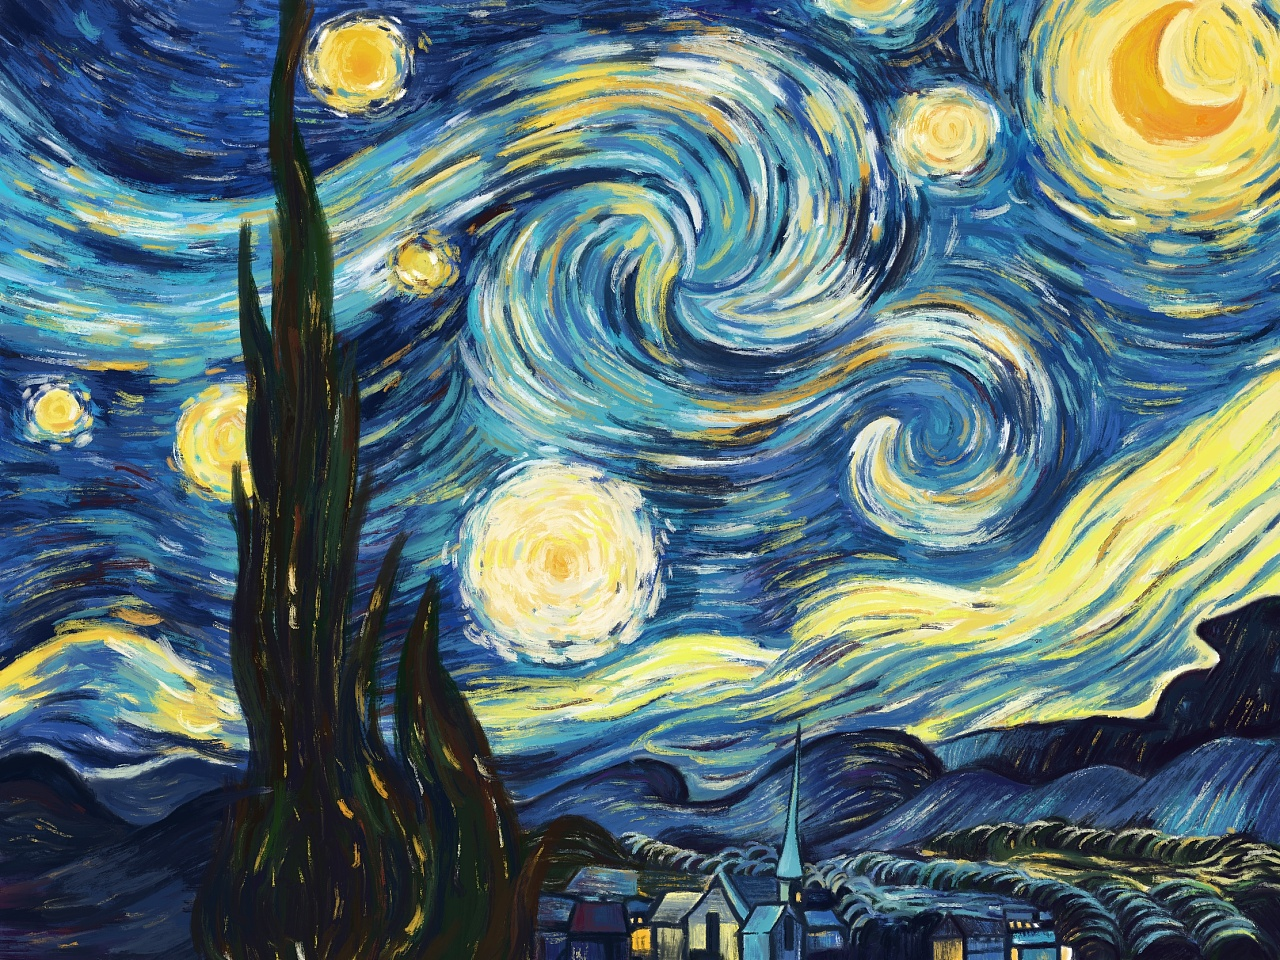
\includegraphics[width=0.9\textwidth]{figures/test}
		\caption{子图1}
	\end{subfigure}
	\qquad
	\begin{subfigure}[t]{0.4\textwidth}
		\centering
		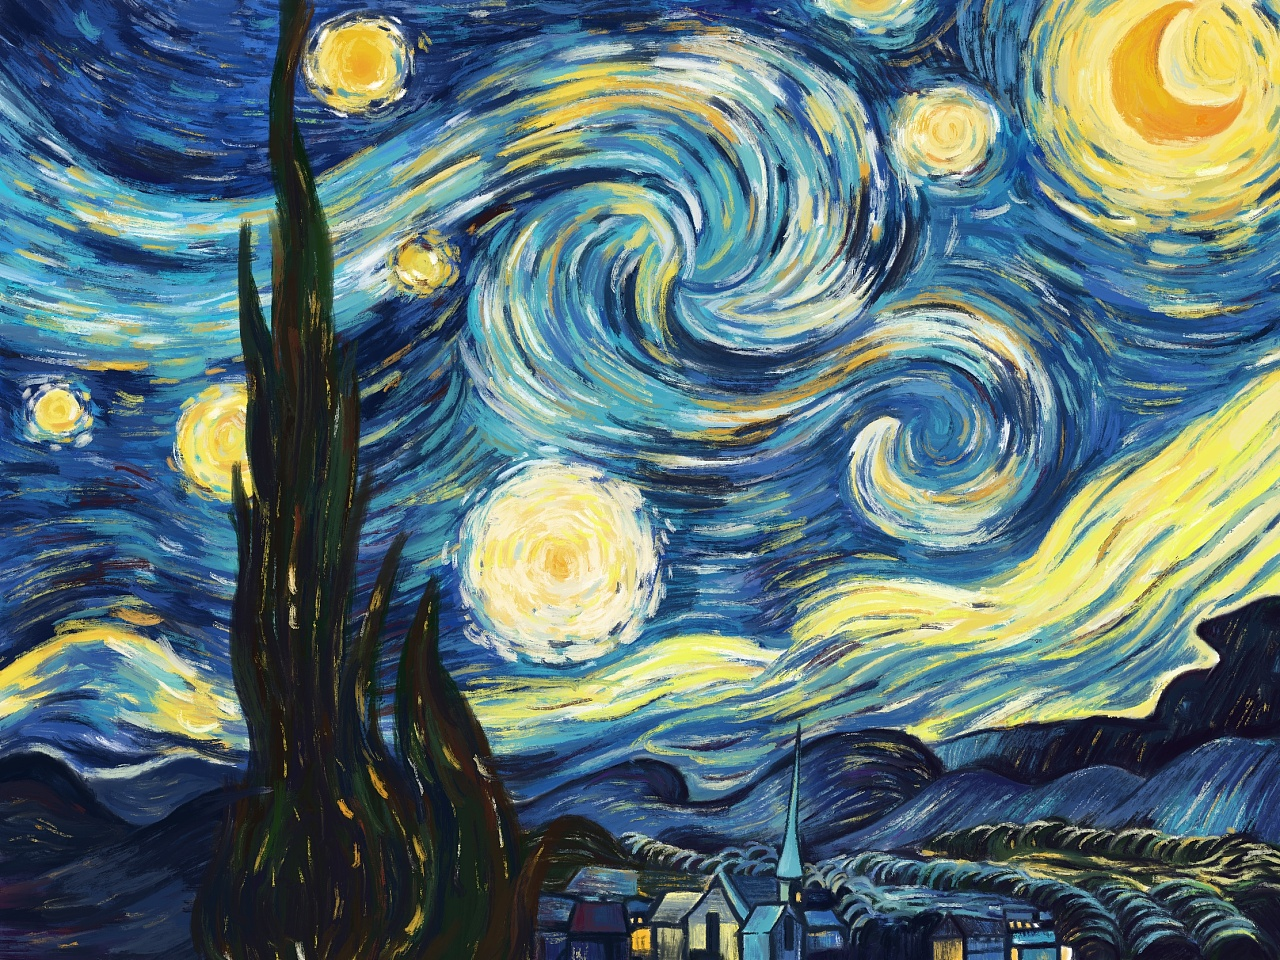
\includegraphics[width=0.9\textwidth]{figures/test}
		\caption{子图2}
	\end{subfigure}
\end{figure}

\begin{lstlisting}[language=tex]
\begin{figure}[htbp]
	\centering
	\begin{subfigure}[t]{0.4\textwidth}
		\centering
		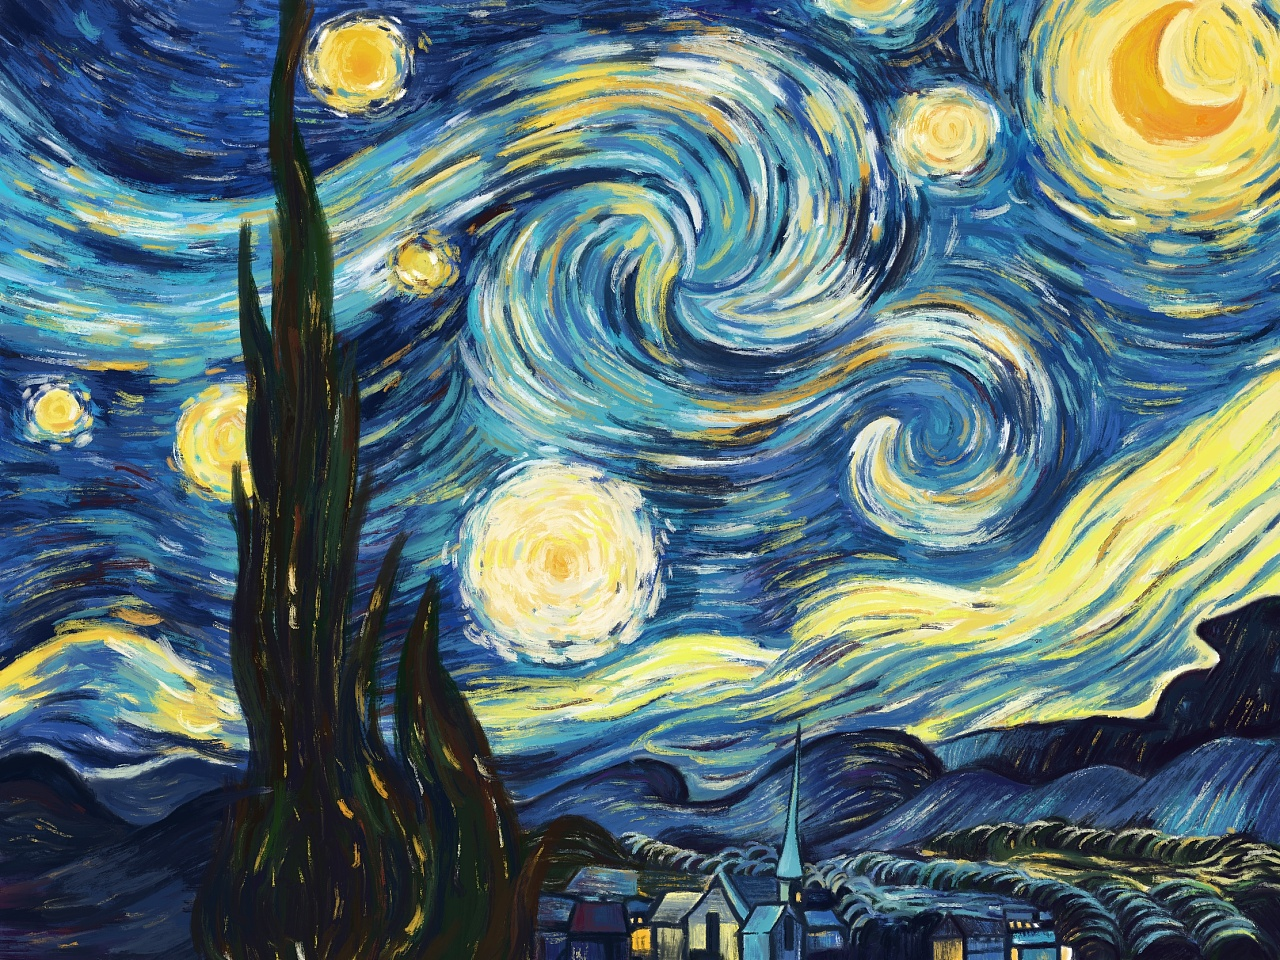
\includegraphics[width=0.9\textwidth]{figures/test}
		\caption{子图1}
	\end{subfigure}
	\qquad
	\begin{subfigure}[t]{0.4\textwidth}
		\centering
		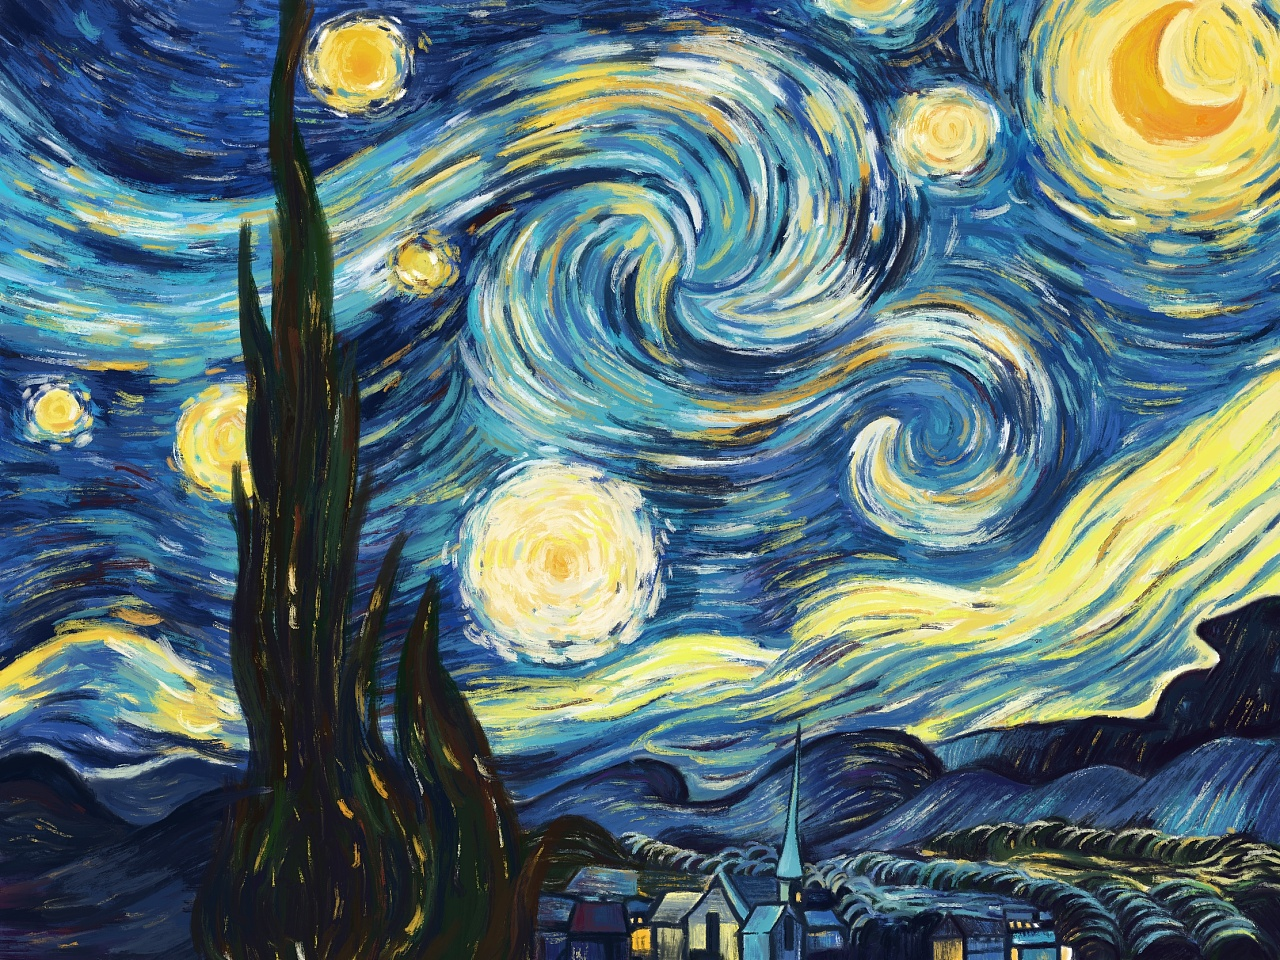
\includegraphics[width=0.9\textwidth]{figures/test}
		\caption{子图2}
	\end{subfigure}
\end{figure}
\end{lstlisting}



